\chapter{\textsc{Methodology}}
\label{chapterlabel4}

The Background chapter provided information about several techniques and concepts that were used throughout the project. This played an important role in the development and analysis process of the project which can be divided into the following stages:

\begin{enumerate}[itemsep=0cm, label*=\arabic*.]
    \item Collection of data from EPSRC
    \item Generation of networks from EPSRC data
    \item Formulation of node and edge attributes
    \begin{enumerate}[itemsep=0cm, label*=\arabic*.]
        \item Normalization of node and edge attribute values
    \end{enumerate}
    \item Comparison of edge weights and community detection algorithms
    \item Identification of an optimal edge weight and community detection\\algorithm
    \item Clustering of Topics and Researchers
    \item Evaluation of of Topic and Researcher clusters
\end{enumerate}

This section provides details regarding the public data provided by EPSRC and its use in this project while it also describes the methods followed during each development and analysis phase.

\section{Data provided by EPSRC}

This project uses data provided publicly by EPSRC through the \textit{EPSRC Grants on the Web (GoW)} service. It consists of current and historical data stored within the Current and Past Grant Portfolio, respectively.

\subsection{EPSRC Grants on the Web (GoW) service}

The Grants on the Web (GoW) service is a web-based facility providing information about research grants funded by EPSRC. The service is updated frequently, and consists of large amounts of information regarding current and historical grants, researchers, panels and quarterly summaries. It also includes search functionality allowing users to search the Web database.

\iffalse
Each record within each entity is detailed within a separate web page. An example of how a Grant record web page looks is presented in Fig. \ref{fig:grant_record} while Fig. \ref{fig:grant_record} represents an example of a Researcher record web page. This project only makes use of the grant and researcher data.
\fi

\subsection{EPSRC Current and Past Grant Portfolio}

The Current and Past Grant Portfolio are sub-facilities of the Grants on the Web (GoW) service providing access to current and historical grant data. Both facilities provide the same kind of information, however the access to information differs slightly. The Past Grant Portfolio requires a time period period to be supplied, and provides grants based on it. This can be a start date, an end date or a start and end date. Fig. \ref{fig:current_grant_portfolio} and Fig. \ref{fig:past_grant_portfolio} present the hierarchical structure of the EPSRC Current and Past Grant Portfolio, respectively.

\begin{figure}[htpb]
    \centering
    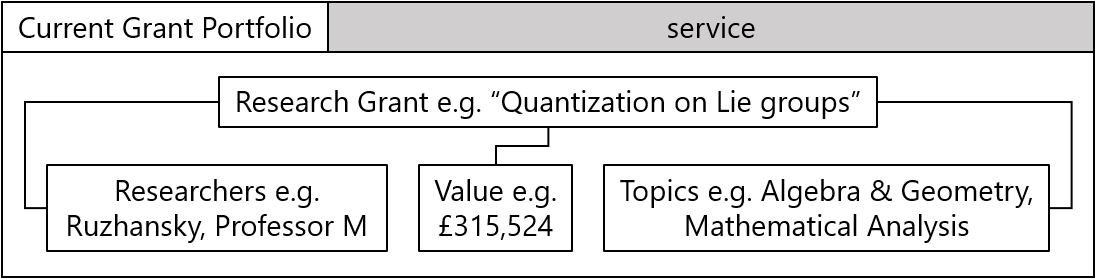
\includegraphics[width=10cm]{portfolios-explained/current_grant_portfolio}
    \caption{Hierarchical structure of the EPSRC Current Grant Portfolio.}
    \label{fig:current_grant_portfolio}
\end{figure}

\begin{figure}[htpb]
    \centering
    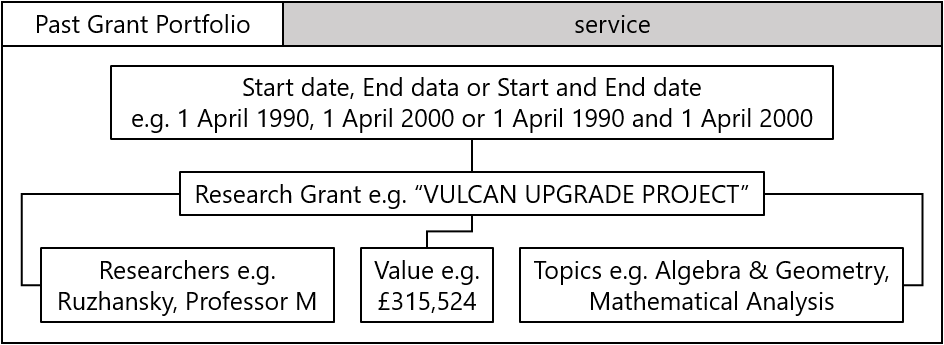
\includegraphics[width=10cm]{portfolios-explained/past_grant_portfolio}
    \caption{Hierarchical Structure of the EPSRC Past Grant Portfolio.}
    \label{fig:past_grant_portfolio}
\end{figure}

Each grant record is stored within a separate web page and contains details about the grant such as \textit{reference}, \textit{investigators (researchers)}, \textit{partners}, \textit{department}, \textit{organisation}, \textit{start} and \textit{end date}, \textit{value} and \textit{topic} and \textit{industrial sector classifications}. Fig. \ref{fig:grant_record} shows an example of a grant record within the \textit{EPSRC Grants on the Web (GoW)} service.

\begin{figure}[htpb]
    \centering
    \fbox{
\includegraphics[width=12cm]{epsrc-records/grant_record}}
    \caption{Grant record within the \textit{EPSRC Grants on the Web (GoW)} service.}
    \label{fig:grant_record}
\end{figure}

The researchers within each grant record are linked to separate researcher records. Each researcher record is also stored within a separate web page and contains details about the researcher including \textit{name}, \textit{organisation}, \textit{department}, \textit{current topics} and \textit{grants}. Fig. \ref{fig:researcher_record} shows an example of a researcher record within the \textit{EPSRC Grants on the Web (GoW)} service.

\begin{figure}[htpb]
    \centering
    \fbox{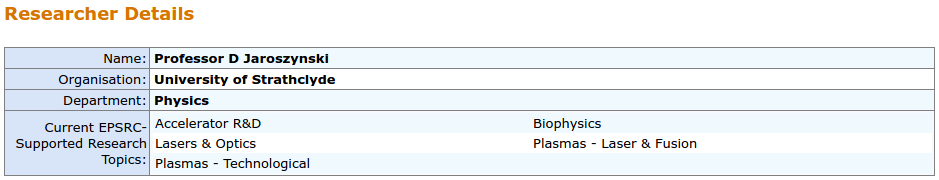
\includegraphics[width=12cm]{epsrc-records/researcher_record}}
    \caption{Researcher record within the \textit{EPSRC Grants on Web (GoW)} service.}
    \label{fig:researcher_record}
\end{figure}

\iffalse
The Current Grant Portfolio within GoW presents data categorised by different research entities such as research area, research topic, theme, industrial sector and so on. This project focuses primarily on research topics, so this entity is used for the following explanation.

The Research Topic page consists of a list of links to different research topics. Within each topic page, a list of links to grants is displayed which related to the topic selected. Each grant page stores information related to the grant such as the researchers working on the grant, the topic classifications of the grant and the value of the grant in British Pounds. Fig. \ref{fig:current_grant_portfolio} illustrates the hierarchical structure of the Current Grant Portfolio.

\begin{figure}[htpb]
    \centering
    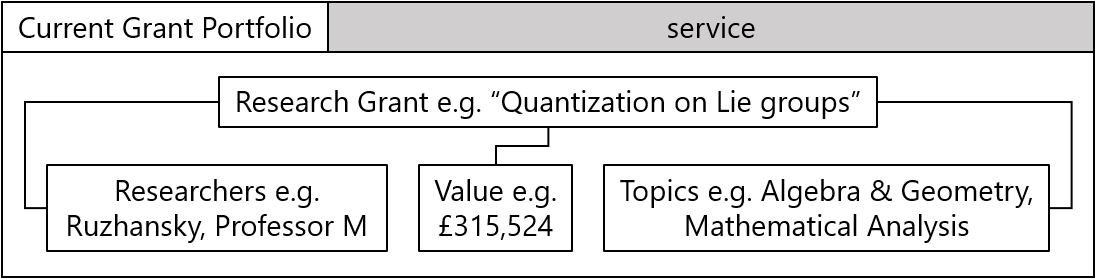
\includegraphics[width=14cm]{portfolios-explained/current_grant_portfolio}
    \caption{Hierarchical structure of the Current Grant Portfolio.}
    \label{fig:current_grant_portfolio}
\end{figure}
\fi

\iffalse
In contrast, the Past Grant Portfolio requires the user to specify a time period and it directly retrieves a list of links to grants based on it. Therefore, the data is only categorised by a time period which represents
either when the grants commenced, completed or commenced and completed. Identically to the Current Grant Portfolio, each grant page stores information including the researchers, topics and value of the grant. Fig. \ref{fig:past_grant_portfolio} illustrates the structure of the Past Grant Portfolio.

\begin{figure}[htpb]
    \centering
    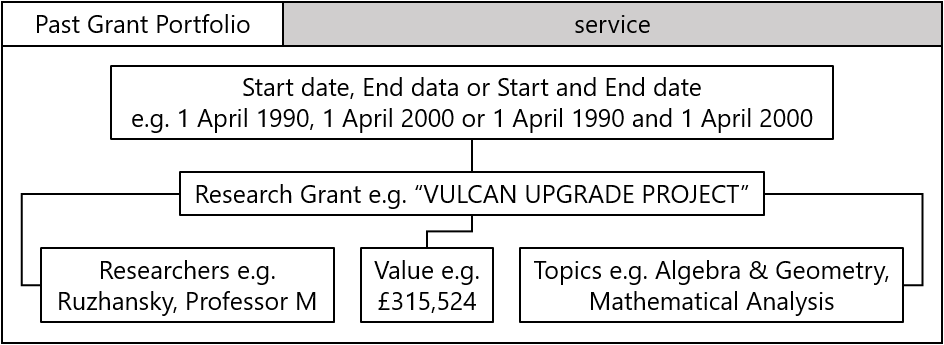
\includegraphics[width=14cm]{portfolios-explained/past_grant_portfolio}
    \caption{Structure of the Past Grant Portfolio.}
    \label{fig:past_grant_portfolio}
\end{figure}
\fi

\iffalse
\subsection{Issues}

For each record, the web scraper has to make a web request, similar to when a user navigates to a web page, and then extract the specified data. For example, to extract data from all current grant records, 3, 175 requests need to be performed. This may not be too problematic, however, for grant data between 2010 and 2000, 18,692 requests are required. Now, that is problematic. Therefore, during the initial process of data extraction, this problem was identified, as the computational time of the past data extraction process was far too lengthy.

Several alternatives were identified as potential solutions to the problem. The scraper could be modified to make asynchronous requests or the physical HTML files could be downloaded and then scraped locally. The latter alternative was chosen, and a script was written in Bash in order to achieve it. This decision was successful and it greatly improved the computational time of the data extraction task.
\fi

\iffalse
\subsection{Process}

In order to extract content from a web page, the page needs to be scraped. This is usually achieved by either using an already built web scraper or by developing a web scraper, which extracts specified data from the underlying tags within the HTML code. In this project, a web scraper was developed using the \textit{requests} and \textit{lxml} Python libraries.

Due to the differences between the Current and Past Grant Portfolios, the data extraction process was also different. All actual data is extracted from either a grant or researcher page. However, to access the grant and researcher pages different series of steps are required depending on whether it is current or past data that is being extracted.

For current data, topic URLs need to be extracted first. Further, the web scraper connects to each topic URL and extracts the grant URLs. Only after the grant URLs are obtained, the web scraper connects to each grant page and begins to extract the actual data. For past data, the process is much simpler as the list of links to grants is supplied directly. This means that the web scraper extracts the grant URLs and then connects to each URLs and starts to extract past grant information. Table \ref{table:data_statistics} presents the number of past and current records within each entity that data was extracted from.

Once extracted, the data is validated and then formatted into a format that allows easy manipulation of it. Finally, it is stored within numerous comma-separated files categorised by content.
\fi

\section{Collection of data from EPSRC}

The previous sections provided an introduction to the data provided by EPSRC, the \textit{Grants on the Web service (GoW)}, the Current and Past Grant Portfolios and the Grant and Researcher records. This project solely uses data collected from the Current and Past Grant Portfolios, and does not use any of the other information provided through the \textit{Grants on the Web (GoW)} service. In terms of the Current and Past Grant Portfolios, this project only makes use of data extracted from grant and researcher records. 

Firstly, data within the following fields of a grant record was extracted:
\textit{EPSRC Reference}, \textit{Principal Investigator}, \textit{Other Investigators}, \textit{Starts}, \textit{Ends} and \textit{EPSRC Research Topic Classifications}. Secondly, data within the \textit{Name} and \textit{Current EPSRC-Supported Research Topics} fields of a researcher record was extracted. 

Furthermore, this project solely extracts the name and current topics from each researcher record. Table \ref{table:grant_researcher_record_numbers} presents the number of current EPSRC grant and researcher records and historical grant records from which data was collected.

Furthermore, this project uses both current and historical data collected from EPSRC, which is organised into two main data sets, while the historical data set is further divided into two sub-data sets as follows:

\begin{itemize}[itemsep=0cm]
    \item \textbf{Current data set}, consisting of current grants (post 2010 start date) and researchers collected on 8 July 2016 
    \item \textbf{Historical data set}, consisting of grant records from two time periods:
    \begin{itemize}[itemsep=0cm]
        \item \textbf{from 1990 to 2000}, consisting of grant records which started and ended between 1 April 1990 and 1 April 2000
        \item \textbf{from 2000 to 2010}, consisting of grant records which started and ended between 1 April 2000 and 1 April 2010
    \end{itemize}
\end{itemize}

\begin{table}[!htbp]
\centering
\caption{Number of current EPSRC grant and researcher records and historical grant records from which data was collected.}
\label{table:grant_researcher_record_numbers}
\begin{tabular}{r|r|r|r}
{} & \multirow{2}{*}{\textbf{Current}}
& \multicolumn{2}{c}{\textbf{Historical}}\\
\cline{3-4}
& {} & \textbf{1990-2000} & \textbf{2000-2010}\\
\hline
\textbf{Number of Grant records}      & {3175} & {17861} & {18692}\\
\textbf{Number of Researcher records} & {5874} & {10820} & {13385}\\
\end{tabular}
\end{table}

The previous section specified that both grant and researcher records are stored as separate web pages within the \textit{Grants on the Web (GoW)} service. In order to extract content from a web page, a technique called \textit{web scraping} is employed. This is usually achieved by either using a third-party web scraper or by developing a web scraper from scratch, which extracts specified data from the underlying tags within the HTML code. In this case, a web scraper was developed using the \textit{requests} and \textit{lxml} Python libraries.

Essentially, the web scraper connects to the URL of each grant and researcher record web page and extracts the text found under specific fields such as \textit{Reference}, \textit{Principal Investigator} and \textit{Other Investigators}, \textit{Value} and \textit{EPSRC Research Topic Classifications}. Once extracted, the data is validated and then comma-delimited and text qualified using quotation marks which preserves its original format and allows easy manipulation of it. Subsequently, it is stored within comma-separated files categorised by content and data set.

\section{Generation of networks from EPSRC data}

In the previous section, the data collection process was explained and documented. The data extracted from the \textit{Grants on the Web (GoW)} service was used to construct several networks of topics and researchers structured as follows:

\begin{enumerate}[itemsep=0cm, label*=\arabic*.]
    
    \item \textbf{Networks of Topics, with nodes representing Topics}
    \begin{enumerate}[itemsep=0cm, label*=\arabic*.]
        \item and edges representing Grants, named \underline{Grants as edges};
            \begin{enumerate}[itemsep=0cm, label*=\arabic*.]
                \item created using the current and historical data sets (1990-2010)
            \end{enumerate}
        \item and edges representing Researchers, named \underline{Researchers as edges};
            \begin{enumerate}[itemsep=0cm, label*=\arabic*.]
                \item constructed using the current data set only\footnote{The Topic (Nodes as Topics, Edges as Researchers) and Researcher network (Nodes as Researchers, Edges as Topics) were created using the Current data set only because Researcher records only consist of a researcher's current topics, and not their historical topics.}
            \end{enumerate}
    \end{enumerate}

    \item \textbf{Networks of Researchers, with nodes representing Researchers}
    \begin{enumerate}[itemsep=0cm, label*=\arabic*.]
        \item and edges representing Grants, named \underline{Grants as edges};
        \begin{enumerate}[itemsep=0cm, label*=\arabic*.]
                \item created using the current and historical data sets (1990-2010)
            \end{enumerate}
        \item and edges representing Topics, named \underline{Topics as edges};
        \begin{enumerate}[itemsep=0cm, label*=\arabic*.]
                \item constructed using the current data set only\footnotemark[1]
        \end{enumerate}
    \end{enumerate}

\end{enumerate}

Node and edge attributes were also formulated and incorporated into the networks. The attribute values "suffered" a normalization process which decreased the scale of the value range. This was followed by extensive experiments which aimed to identify an optimal edge weight and community detection algorithm. Several edge weights (\textit{unweighted}, \textit{weighted by normalized number of projects} and \textit{weighted by normalized value of projects}) and community detection algorithms (\textit{Spinglass}, \textit{Louvain}, \textit{Fast Greedy}) were considered. The optimal solution was chosen based on the modularity score and coherence of the generated topic and researcher clusters.

This section describes how the collected data was used further in the next phase of development including network generation and topic and researcher clustering.

\subsection{Networks of Topics}

The concept of the topic-based network involved two potential ways that the network could be constructed. The topics could be analysed from the perspective of grants as well as researchers. This resulted in the creation of two different networks of topics. In both networks, nodes represent topics. However, edges represent either grants or researchers. For ease of reference, the two networks will be referred to as \textit{Grants as edges} and \textit{Researchers as edges}, respectively.

\subsubsection{Topic network (Grants as edges)}

This network consists of nodes representing topics and edges representing grants. An edge between two nodes means that two topics have a grant in common. Each grant record consists of a \textit{EPSRC Research Topic Classifications} field consisting of research topics that classify the grant. In order to achieve the creation of this network, grants with two or more topics had to considered. For each grant record, an edge was "drawn" between each of the topics. Fig. \ref{fig:topic_a_structure} provides a visual explanation of the network's structure. The network consists of two node and edge attributes, number and value of grants. Furthermore, the node and edge attributes are explained further in the \textit{Node and Edge attributes} section.

\begin{figure}[!htbp]
    \centering
    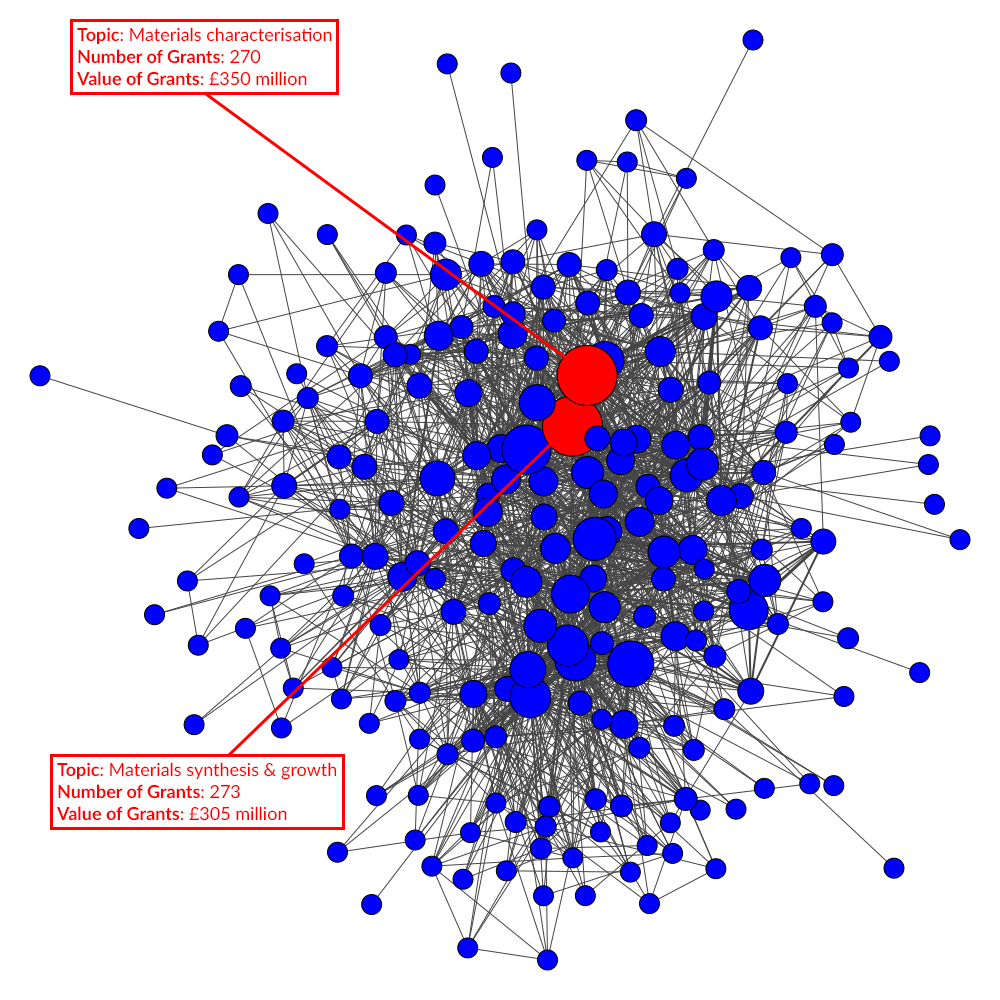
\includegraphics[width=7cm]{networks-explained/topic_network_a}
    \caption{Visual explanation of how the Topic network (Grants as edges) was constructed including the formulated node and edge attributes.}
    \label{fig:topic_a_structure}
\end{figure}

\subsubsection{Topic network (Researchers as edges)}

This network consists of nodes representing topics and edges representing researchers. An edge between two nodes means that two topics have a researcher in common. Each researcher record consists of a \textit{Current EPSRC-Supported Research Topics} field consisting of the researcher's current research topics. In order to achieve the creation of this network, researchers with two or more current topics had to be considered. For each researcher record, an edge was "drawn" between each of the topics. Fig. \ref{fig:topic_b_structure} provides a visual explanation of the network's structure. Furthermore, the network consists of a node and edge attribute, number of researchers. The formulation of node and edge attributes is explained in detail in the \textit{Node and Edge attributes} section.

\begin{figure}[!htbp]
    \centering
    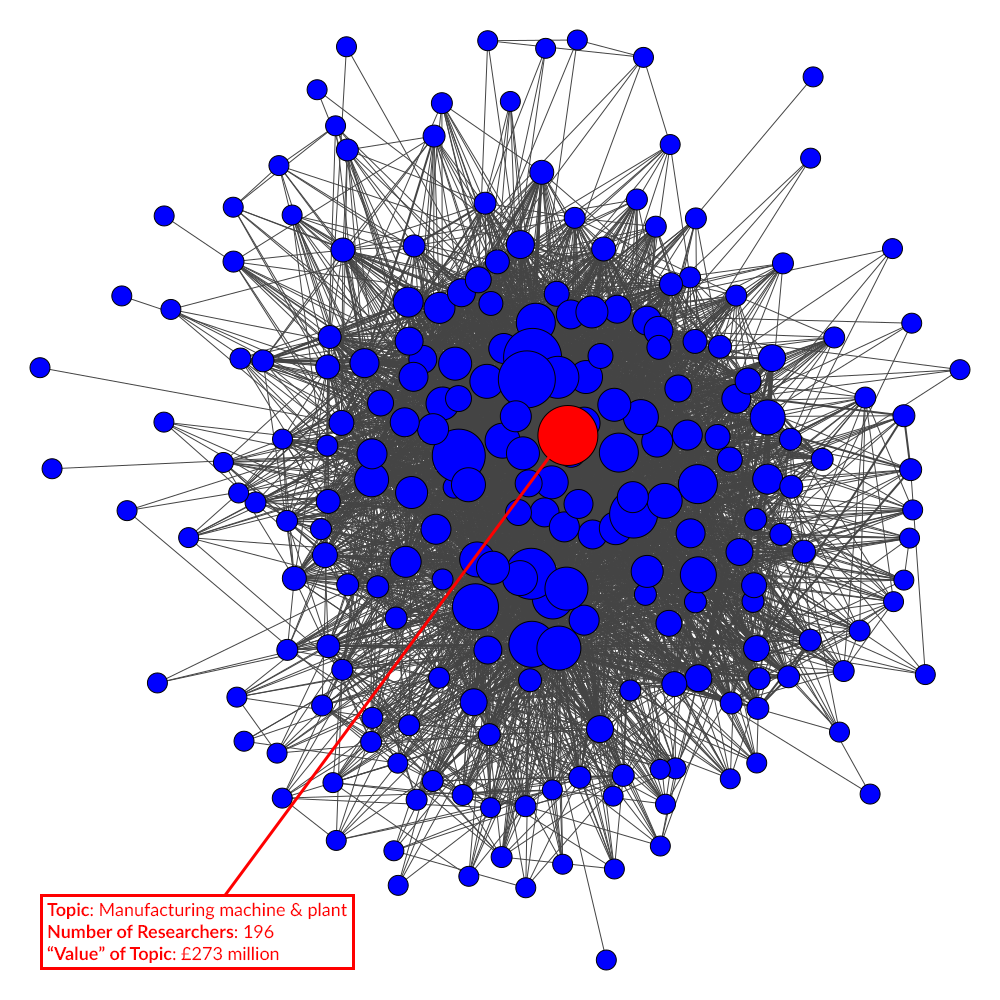
\includegraphics[width=8cm]{networks-explained/topic_network_b}
    \caption{Visual explanation of how the Topic network (Researchers as edges) was constructed including the formulated node and edge attributes.}
    \label{fig:topic_b_structure}
\end{figure}

\subsection{Networks of Researchers}

The concept of the researchers network involved two potential ways that the network could be constructed. The researchers could be analysed from the perspective of grants as well as topics. This resulted in the creation of two different networks of researchers. In both networks, nodes represent researchers. However, edges represent either grants or topics.  For ease of reference, the networks will be referred to as \textit{Grants as edges} and \textit{Topics as edges}, respectively.

\subsubsection{Researcher network (Grants as edges)}

This network consists of nodes representing researchers and edges representing grants. An edge between two nodes means that two researchers have a grant in common. Each grant record consists of the \textit{Principal} and \textit{Other Investigators} fields consisting of researchers collaborating on the grant. In order to achieve the creation of this network, grants with two or more researchers were considered. For each grant record, an edge was "drawn" between each of the researchers. Fig. \ref{fig:researcher_a_structure} provides a visual explanation of the network's structure. Due to the significantly large size of the \textit{Researcher network (Grants as edges)}, the network had to be sampled with the sample consisting of nodes connected by edges with an edge weight of 2 or more. Furthermore, the network consists of two node and edge attributes, number and value of grants. The formulation of node and edge attributes is explained in detail in the \textit{Node and Edge attributes} section.

\begin{figure}[htpb]
    \centering
    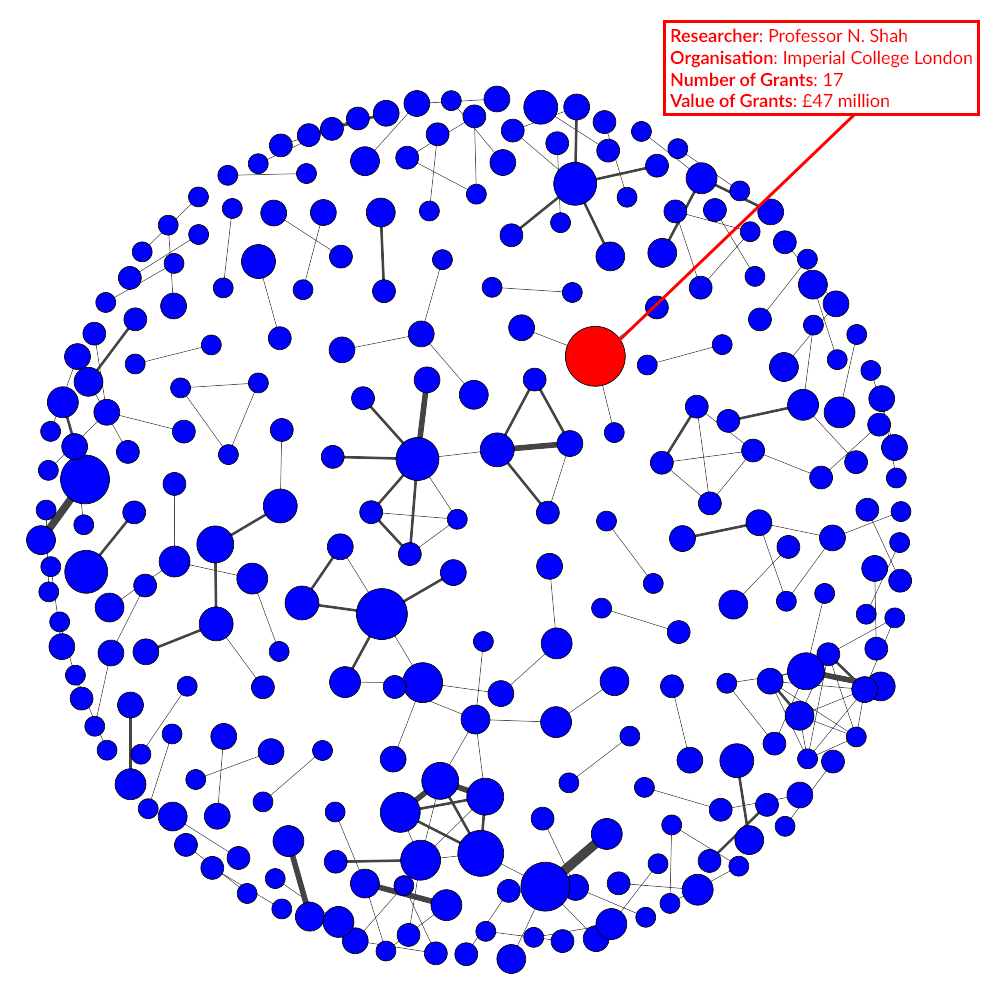
\includegraphics[width=8cm]{networks-explained/researcher_network_b}
    \caption{Visual explanation of how the Researcher network (Grants as edges) was constructed including the formulated node and edge attributes.}
    \label{fig:researcher_a_structure}
\end{figure}

\subsubsection{Researcher network (Topics as edges)}

This network consists of nodes representing researchers and edges representing topics. An edge between two researchers means that two researchers have a topic in common. Each researcher record consists of a \textit{Current EPSRC-Supported Research Topics} field consisting of the researcher's current research topics. In order to achieve the creation of this network, each researcher was compared to all other researchers and if they had at least one topic in common, an edge was "drawn" between the researchers. Fig. \ref{fig:researcher_b_structure} provides a visual explanation of the network's structure. Due to the significantly large size of the \textit{Researcher network (Topics as edges)}, the network had to be sampled with the sample consisting of nodes connected by edges with an edge weight of 5 or more. Furthermore, the network consists of a node and edge attribute, number of topics. The formulation of node and edge attributes is explained in detail in the \textit{Node and Edge attributes} section.

\begin{figure}[htpb]
    \centering
    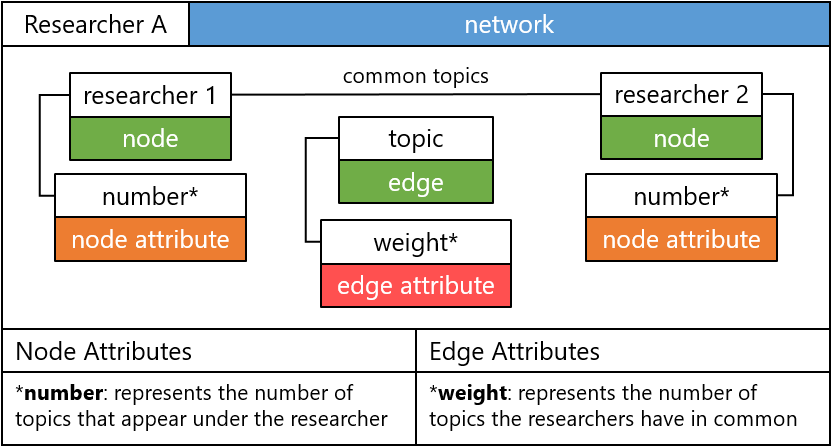
\includegraphics[width=8cm]{networks-explained/researcher_network_a}
    \caption{Visual explanation of how the Researcher network (Topics as edges) was constructed including the formulated node and edge attributes.}
    \label{fig:researcher_b_structure}
\end{figure}

\subsection{The contrast between grants as edges and grant records}

It is essential to point out that there is a clear difference between grants represented by edges and the actual grant records that appear on the \textit{Grants on the Web (GoW)} service. First and foremost, the former is not unique within a network, while the latter is unique within the GoW service. This is because of the way links between topics or researchers were established in a network. For example, if a grant is classified by three topics, each topic is linked to one another by a separate edge, which represents the common grant in question. Therefore, in this case, three edges are created to link the topics which represent the same common grant, meaning that the grant will appear within the network three times. It is also crucial to specify that unlike grants, a network consists of nodes representing unique topics.

This causes issues when questions like the following are posed: \textit{How many grants are in a specific community within a network's community structure?} \textit{What is the value of the grants?} It is important to mention that it is not known which grant is represented by an edge. It is only known that it represents one or more grants depending on the edge weight. If this was known, providing an answer to the above questions becomes significantly easier. In contrast, the answer was achieved through a lengthier process. Furthermore, the edges linking topics within the same community and the edges linking topics in different communities were known. This greatly aided the identification process of both the number and value of grants within communities and between communities.

Firstly, the origin and destination topics of an edge within a network were retrieved. Secondly, during the data collection process, a data structure was created which stored the reference of each grant and the topics that classify it. Next, a check was carried out against all grant records which verified whether both the retrieved origin and destination topics appeared under a grant record. Number and value counters were created to keep track of the cumulative number and value of grants. When the check was true, the reference and value of the grant were added as the key and value to a Python dictionary, in which all keys must be unique. Finally, at the end of the check, the number of grant references was counted and the grant values were summed up. This provided an answer to the questions asked, as the number and value of grants within a community was successfully identified. Additionally, using the same technique, the computation of the number and value of grants between communities and within the entire network was also achieved. The function written in order to achieve this task can be viewed in Code snippet \ref{listing:turn_edges_into_grants} within Appendix \ref{appendix:code}.

\subsection{Formulation of node and edge attributes}

Every network constructed using the data collected from EPSRC consists of at least one node and edge attribute, while others consist of two attributes. Both \textit{Topic} and \textit{Researcher networks (Grants as edges)} consist of a \textit{number} and \textit{value} attribute, while the \textit{Topic (Researchers as edges)} and \textit{Researcher (Topics as edges)} networks only consist of a \textit{number} attribute. Visually, the network attributes control both the size of the node circle and the thickness of the edge line. This section documents the formulation of the node and edge attributes, which allow the analysis and visualisation of the network from two different perspectives.

\subsubsection{Number of grants/topics/researchers}

The number attribute has a number of different contexts, depending on the network. Firstly, in the \textit{Topic} and \textit{Researcher networks (Grants as edges)}, the node number attribute represents the number of grants that contain a topic or researcher. In the same networks, the edge number attribute represents the number of grants two topics or researchers have in common, meaning they are both contained within the same grant record. Secondly, in the \textit{Topic network (Researchers as edges)}, the node number attribute represents the number of researchers that contain the topic, while the edge number attribute represents the number of researchers two topics have in common, meaning they are both contained within the same researcher record. Thirdly, in the \textit{Researcher network (Topics as edges)}, the node number attribute represents the number of topics a researcher currently has, while the edge number attribute represents the number of topics two researchers have in common.

\subsubsection{Value of grants}

Similarly, the value attribute also has a number of different contexts, depending on the network. Firstly, networks that are not based on grant data do not contain of the value attribute. Secondly, in the \textit{Topic} and \textit{Researcher network (Grants as Edges)}, the node value attribute represents the value of a topic or researcher. This represents the value of the grants that contain that specific topic or researcher. In the same network, the edge value attribute represents the value of the grants that two topics or researcher have in common, meaning they are both contained within the same researcher record.

\subsection{Normalization of node and edge attribute values}

The numerical values used as the node and edge attributes, especially the value attribute, represent significantly large numbers which cause issues in terms of development, analysis and visualisation. To accommodate this, the values underwent a normalization process which scaled the value range down. The function written in order to achieve this task can be viewed in Code snippet \ref{listing:norm_vals} within Appendix \ref{appendix:code}, while the formula used to normalize the values is presented below:

\begin{equation}
    (val - old\_min) \times new\_range / old\_range) + new\_min)
\end{equation}
where:
\begin{itemize}[itemsep=0cm]
    \item \textit{val} is the value being normalized
    \item \textit{old\_min} is the minimum of the initial value range
    \item \textit{new\_range} is the new range values will be normalized to
    \item \textit{old\_max} is the maximum of the initial value range
    \item \textit{new\_min} is the minimum of the new value range
\end{itemize}

\section{Comparison of edge weights and community detection algorithms}

In the previous section, the process carried out to normalize the values used as node and edge attributes was described. This section details the experiments carried in order to identify the most coherent division of the topic and researcher networks into topic and researcher clusters.

Several experiments were carried seeking to identify an optimal edge weight and community detection algorithm that produced the most rational clustering results. In order to ensure a consistent analysis, the experiments were solely carried out on the \textit{Topic} and \textit{Researcher network (Grants as edges)}. The results of the experiments on this network were applied to all the other networks.

Eight different community detection algorithms were considered including \textit{Louvain}, \textit{Spinglass} and \textit{Fast Greedy}. The \textit{Topic network (Grants as edges)} consists of two node and edge attributes, number and value of grants. The values of both attributes are significantly large and therefore they were normalized for development, analysis and visualisation purposes. In total, three different "candidates" of interpreting the edge weight were considered: \textit{unweighted}, \textit{weighted by normalized number of grants} and \textit{weighted by normalized value of grants}.

Furthermore, the eight community detection algorithms were applied to each network using each of the three edge weight interpretations, while the results of the experiments underwent a multi-phase comparative analysis, documented in the next section.

\section{Identification of an optimal edge weight and community detection algorithm}

The experimental stage consisted of a number phases. In the first phase, a number of community detection algorithms were applied to the network using each of the edge weight interpretations. The resulting modularity scores and number of generated communities were compared across all edge weight and community detection algorithm candidates. Most community detection algorithms make use of the edge weight attribute in the clustering process, which meant that the \textit{unweighted} edge weight interpretation had a low-performance and was excluded from the tests in the first phase. Furthermore, a number of community detection algorithms such as \textit{Label Propagation}, \textit{Leading Eigenvector} and \textit{Edge Betweenness} were also excluded due to low performance results. In contrast, the \textit{Louvain}, \textit{Spinglass} and \textit{Fast Greedy} algorithms remained to be tested further.

During the second phase, the number of topics within each community was compared across all candidates, and it was decided that all remaining edge weight interpretations and community detection algorithms would proceed to the final testing phase. In the third phase and the final phase, each community of topics identified using each one of the edge weight interpretations and community detection algorithms were compared to each other based on coherence and balance. Finally, it was concluded that the clustering produced by the \textit{normalized number of grants/topics/researchers} edge weight interpretation and the \textit{Louvain} community detection algorithm was the most reasonable and the one that would be employed throughout the rest of the analysis.

\section{Clustering of Topics and Researchers}

As revealed in the previous section, the \textit{Louvain} community detection algorithm performed the best when applied to a network in which the weight of an edge represents the \textit{normalized number of grants, topics or researchers}. Following this discovery, the identified combination of edge weight and community detection algorithm was considered the optimal solution.

Furthermore, the solution was applied to each network in order to identify its underlying community structure. This resulted in a number of communities also known as clusters or groups, consisting of topics or researchers. Each topic or researcher was assigned to exactly one cluster. Certain identified communities can be quite broad in terms of the representation of research areas, especially if the network consists of a large number of nodes. In order to achieve a more specific clustering, the community detection algorithm was applied to each previously identified community in order to discover its sub-communities which form each community's underlying community structure.

Moreover, the topic and researcher clustering was documented in a Microsoft Excel spreadsheet. The number and value of grant records in each community was also documented and calculated. This was followed by the creation of word cloud representations of the communities and sub-communities identified within the \textit{Topic network (Grants as edges)}, using Wordle. Each community and sub-community was illustrated from three different perspectives: \textit{word frequency}, \textit{number of grants} and \textit{value of grants}.

\section{Evaluation of Topic and Researcher clusters}

Once the topic and researcher clusters were identified and defined, they underwent an evaluation stage which determined how strong the links between nodes in the same clusters are compared to links that connect nodes that are in different clusters. This was achieved by calculating the Dice and Jaccard similarity of nodes within the same and different clusters.

Firstly, the origin and destination nodes of each edge in the network were identified. This forms a pair of nodes as follows: origin node, destination node. Certain edges connect nodes that are in the same cluster, while others link nodes that are in different clusters. Therefore, some node pairs represent nodes from the same cluster, while others represent nodes from different clusters. Secondly, the Dice and Jaccard similarity between each node pair was calculated. Theoretically, a pair of nodes from the same cluster should be more similar than a pair of nodes from different clusters. The evaluation phase helped to determine whether in reality this is also true. Finally, in order to obtain an overall perspective of the similarity of nodes within and between clusters, the average Dice and Jaccard similarity was calculated.

\section{Tools used in this project}

During this study, several tools were employed in order to accomplish various development and analysis activities. This section describes the tools and comments on their use throughout the project.

\subsection{JetBrains PyCharm used for programming}

JetBrains PyCharm \cite{jetbrains_pycharm} is an Integrated Development Environment (IDE) for programming in Python. It also provides support for writing code in Bash. It was used to write the development code in primarily Python but also in Bash.

\subsection{Microsoft Excel used for data storage}

Microsoft Excel \cite{microsoft_excel} is a spreadsheet software featuring calculation, graphing tools, pivot tables, and macro programming support in Visual Basic. It was used to explore, filter and validate the collected data.

\subsection{iGraph used for network analysis and visualisation}

iGraph \cite{csardi2006igraph} is a library collection for creating and manipulating graphs and analyzing networks. This tool was used to compute network properties, apply community detection algorithms, and produce visualisations of the networks created.

\subsection{NetworkX used for visualising adjacency matrices}

NetworkX \cite{networkx} is a package for the creation, manipulation, and study of the structure, dynamics, and functions of complex networks in Python. It was used to visualise adjacency matrices.

\subsection{Wordle used for creating word cloud visualisations}

Wordle \cite{wordle} is a tool for visualising text as word clouds. By default, it computes each word's frequency and displays the more frequent words in a larger font than less frequent ones. Additionally, Wordle's advanced mode allows keeping words together, specifying a weight which control the font size as well as specifying a colour for each word. It was to create word cloud representations of topic clusters using several attributes to control font size and colour.

\subsection{Adobe Photoshop used for image editing}

Adobe Photoshop \cite{adobe_photoshop} is a graphics editor developed by Adobe Systems. It was used for image editing as well as turning network plots produced using iGraph into complete network visualisations.